% !TEX root = ../../report.tex

\section{Recommender Systems foundations}
\label{sec:recsys}
Recommender systems have become an important research topic since the
introduction of Tapestry \cite{Goldberg1992}, the first collaborative filtering
system back in 1992. Recommender systems now play an important role in many of
the most popular web-sites such as Amazon, YouTube, Netflix, TripAdvisor,
Last.fm, and IMDb. In its most common formulation the recommendation problem is
reduced to the problem of estimating the preference/rating of items that have
not been seen by a user. Usually, this estimation is based on one or more of
the following assumptions:

\begin{itemize}
\item You are like your friends
\item You are like people who do similar things that you do
\item You like things that are similar to things you already like
\item You are influenced by experts and the opinions of others.
\end{itemize}

Once we have estimated these ratings we can recommend the items with the
highest rating to the user. These recommendations relate to various
decision-making processes, such as what items to buy, what music to listen to,
or what online news to read. Recommender systems are usually classified into
the following categories, based on how the recommendations are made
\cite{Adomavicius2005}.

\begin{itemize}
\item \emph{Content-based recommendations:} The user will be recommended items with similar content to the ones the user preferred in the past;
\item \emph{Collaborative recommendations:} The user will be recommended items that people with similar tastes and preferences have liked in the past;
\item \emph{Hybrid approaches:} These methods combine collaborative and content-based methods.
\end{itemize}

\subsection{Content Based Filtering}

In a content-based system, we must construct a user \emph{profile}
$ContentBasedProfile(c)$ or each user $c$, which is a record or collection of
the attributes which characterizes each item $Content(s)$ of all the items
$s_{i} \epsilon S$ previously rated by user $c$. For example in a fashion
recommender system the content-based recommender system tries to understand the
commonalities among the items user $c$ has rated highly in the past (color,
brand, store, price, etc.). Then recommend items that have a high degree of
similarity to these items. $ContentBasedProfile(c)$ can be designed as a vector
of weights $(w_{c1} ... w_{ck})$, where each weight $w_{ci}$ denotes the
importance of the keyword $k_{i}$ to user $c$.

Items that can be recommended to the user can often be stored in a database
table. Figure \ref{figure:contentbaseddb} shows a simple database with rows
describing 5 items that have been rated by 3 users. The column names starting
with $X_{n}$ are the properties of the items, often referred to as
"attributes".

\begin{figure}[H]
    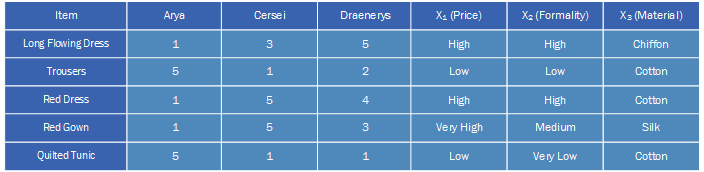
\includegraphics[width=5in]{image/contentbaseddb.png}
    \centering
    \caption[A clothing database]{A clothing database. Rows are items, columns are users and item attributes}
    \label{figure:contentbaseddb}
\end{figure}

From the rating matrix and content properties one can then construct a
$ContentBasedProfile(c)$ for each user $c$, for the user Arya one could imagine
it would look something like this.

\begin{figure}[H]
    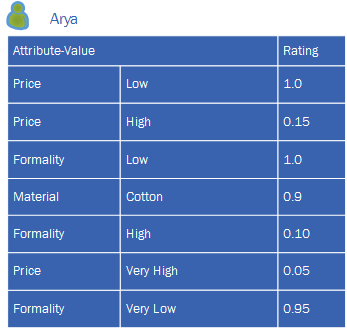
\includegraphics[width=2in]{image/contentprofile.png}
    \centering
    \caption[Content Profile Example]{Content Profile Example}
    \label{figure:contentprofile}
\end{figure}

The recommendation process consists of matching up the attributes of the user
profile against the attributes of an item. The result is a relevance judgment
that represents the user's level of interest in that object. The utility $u(c,
s)$ of item $s$ for user $c$ is estimated based on the utilities $u(c, s_{i})$
assigned by user c to items $s_{i} \epsilon S$ that exhibit a similarity to
item $s$. E.g. for the user Arya items with the attributes low price and low
formality could safely be recommended as they fit her user profile, and have
similar characteristics to the items which she previously have rated highly.
The utility function $r(u, i)$ is usually defined as:

\begin{equation}
r(u,i) = score(ContentBasedProfile(u), Content(i)).
\end{equation}

\subsection{Collaborative Filtering}
\label{subsec:cf}

The goal of collaborative filtering methods is to suggest new items or to
predict the utility $u(c, s)$ of a certain item $s$ for a particular user $c$ based
on the user's previous activities and/or likings and similarity to other users~\cite{Sammut:2011:EML:2011878}.
In a typical CF scenario, there is a list of $n$ users $C = {c_{1}, ... c_{n}}$
and a list of $m$ items $S = {s_{1},...s_{m}}$. Each user $c_{i}$ has a list of
items $S_{si}$, which the user have expressed her opinion about, which makes up
our rating matrix of size $S \times C$. More formally, the utility $u(c, s)$ of
item $s$ for user $c$ is estimated based on the utilities $u(c_{j}, s)$
assigned to item $s$ by the users $c_{j} \epsilon C$, which can be considered
"similar" to the active user $c$. This is exemplified in Figure
\ref{figure:ratingmatrix}. For example, in our fashion recommender system, in
order to recommend clothes to user $c$, the collaborative filtering method must
find the "peers" of users $c$, which share the same tastes in clothes (user
which tend to enjoy similar clothes). Then, recommend the clothes that are most
liked among these "peers".

\begin{figure}[H]
    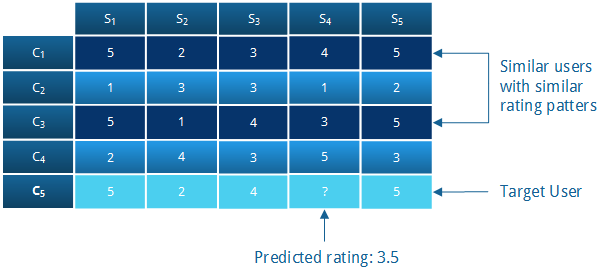
\includegraphics[width=5in]{image/ratingmatrix.png}
    \centering
    \caption[Collaborative filtering rating matrix]{Collaborative filtering rating matrix}
    \label{figure:ratingmatrix}
\end{figure}

Researchers have devised a number of collaborative filtering algorithms that
can be divided into two main categories: Memory-based and Model-based
algorithms \cite{Su2009}.\linebreak[4]

\begin{figure}[H]
    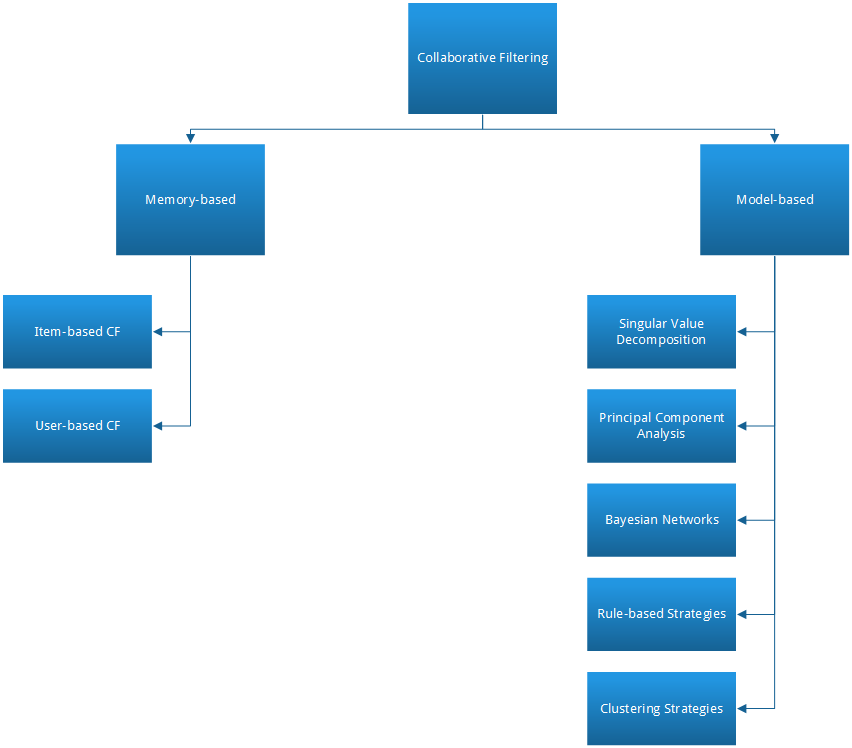
\includegraphics[width=5in]{image/cftaxonomy.png}
    \centering
    \caption[Classification of collaborative filtering techniques]{Classification of collaborative filtering techniques}
    \label{figure:cftaxonomy}
\end{figure}

\subsubsection{Memory-based Methods}
\marginpar{Change to Neighborhood models?}
\marginpar{Make clearer distinction between user-based and item-based}

Memory-based Collaborative Filtering methods utilize the entire user-item
database to generate predictions~\cite{Lin1994}. More formally, the value of an unknown
utility $u(c,s)$ for user $c$ and item $s$ is usually computed by taking the
weighted average of the utilities assigned by the $N$ most similar users for
the same item $s$. The similarity between user $c$ and $c'$, $sim(c, c')$ is
used as the weight. The more similar a user $c'$ is to $c$, the more weight is
given to the utility $u(c', s)$, and thus, will carry more weight in the
prediction for $u(c,s)$.

\begin{equation}
\label{equation:cfratingprediction}
u(c,s) = k * \sum_{c' \epsilon C} sim(c, c') * u(c',s)
\end{equation}

where k serves as a normalization factor, usually being $1/|C|$. Various
approaches have been used to compute the similarity $sim(c, c')$ between the
users. Generally these approaches are based on the rating similarities for
items both users have rated. The most popular similarity measure is The Pearson
Correlation Coefficient. Equation \ref{equation:pearson} shows how to calculate
the Pearson Correlation Coefficient between two users $c$ and $c'$, Here
$S_{cc'}$ is the set of items both users have in \emph{common}.

\begin{equation}
sim(c, c') = \frac{\sum_{s \epsilon S_{cc'}} (u(c, s)-\bar{u_{c}})(u(c',s)-\bar{u_{c'}})}{\sqrt[•]{\sum_{s \epsilon S_{cc'}} (u(c, s)-\bar{u_{c}})^{2}(u(c',s)-\bar{u_{c'}})^{2}}}
\label{equation:pearson}
\end{equation}

Where $u_{c}$ is the mean utility of user $c$. The Pearson Correlation
Coefficient and other similarity measures such as cosine based approaches are
more commonly known user-based collaborative filtering. This is often harder to scale because of the dynamic nature of users. \newline

Item-based Top-N Recommendation methods calculates the similarity between items
instead of users. In these approaches, the historical information is analyzed
to identify the relations between items such that a purchase of another item
(or set of items) often leads to the purchase of another item. These models are
often used since they quickly can recommend a set of items, and have shown to
produce recommendation results comparable or better than traditional user-based
approaches \cite{Karypis2001}.

The algorithm first computes the $k$ most similar items for each item according
to the ratings given by users they both share. Once the most similar items are
found, the prediction is then computed by taking the weighted average of the
target user's ratings on these similar items.

\begin{equation}
u(c,s) = \frac{\sum_{all similar items, S} (sim(s,S)u(c, S)}{\sum_{all similar items, S}(|s,S|)}
\end{equation}

Items that often are rated similarly by users are considered more similar than
items which share few similar ratings. Figure \ref{figure:itemsim} illustrates
the process of finding the item-similarities.

\begin{figure}[H]
    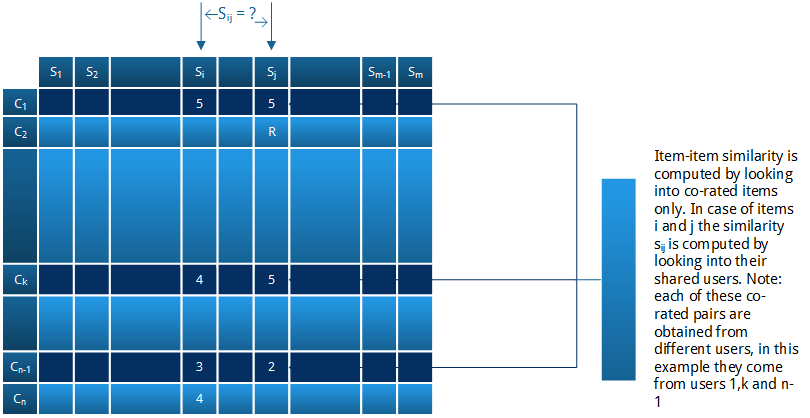
\includegraphics[width=5in]{image/itemsim.png}
    \centering
    \caption[Item-item similarity]{Item-item similarity}
    \label{figure:itemsim}
\end{figure}

There are a number of ways of computing the similarity between items. E.g. by
means of cosine-based similarity. In this case, two items are though of as two
vectors in an $C$ dimensional user space. The similarity between the items is
found by computing the cosine of the angle between the two vectors.

\begin{equation}
sim(s',s) = cos(\vec{s'},\vec{s}) = \frac{\vec{s'} \cdot \vec{s}}{\|\vec{s'}\|^{2} * \|\vec{s}\|^{2}}
\end{equation}

The item similarities can then used to find the Top-N recommendations. Each
user has a set of items $S_{c}$ previously rated by the user which we want to
compute top-N recommendations for. First, we identify the set $C$ of candidate
items recommended items by taking the union of the $k$ most similar items and
removing each of the items in the set $S_{c}$ the user already has rated; then
calculate the similarities between each item of the set $C$ and the set
$S_{c}$, using only the $k$ most similar items for each item in $S_{c}$. The
resulting set of items in $C$ are sorted in descending order of similarity and
will be the recommended as the item-based Top-N list \cite{Karypis2001}.
Items usually do not change as much as users, so this can often be computed offline.
Linden et al \cite{Linden2003} showed that item-based neighborhood methods also provide 
another advantage over other methods, such as e.g. user-based neighborhood models:
in many industrial systems, most of the recommendation is made by the contextual 
recommendation to anonymous users, as on the Amazon's website \marginpar{Add footnote}. This 
recommendation is called item-to-item recommendation, and generally includes the archetype 
associated message "people who have seen / bought this item also viewed / purchased these items. 
This recommendation is directly based on an item-item similarity matrix on click or 
purchase logs.

\subsubsection{Model-based Methods}
\label{model-based-methods}

As the name implies, Model-based approaches provide recommendations by first
developing a model of the user ratings, which is then used to make predictions~\cite{Su:2009:SCF:1592474.1722966}.
These algorithms develop a model of user ratings rather than identify a
neighborhood of similar users or items. These models can be built using various
strategies, such as Singular Value Decomposition (SVD), Principal Component
Analysis (PCA), Rule-based Strategies, Clustering Strategies and Bayesian
Networks.

Latent factor models is probably the most representative approach. Latent
factor models transform both items and users to a latent factor space. The
latent factor space tries to explain the ratings by characterizing both items
and users on factors automatically inferred from the data. The most popular
latent factor models are based on matrix factorization techniques
\cite{Koren2009}.

The main idea behind matrix factorization is just as its name implies,
factorize a matrix, finding two or more matrices such that when you multiply
them you get back the original matrix. Matrix factorization can be used to
discover latent factors underlying the interactions between the users and
items. These factors \emph{explain} how a user rates an item (i.e. that a user
would give high ratings to a certain shirt if he likes the brand, or if the
color is nice). If we can discover these factors, we should be able to predict
a rating with respect to a certain user and a certain item based on the
correlation between their factors.

A matrix factorization model map both users and items to a joint latent factor
space of dimensionality $f$, where $f$ is the number of latent factors. The
number of latent factors are usually determined by using a hold-out dataset or
cross-validation by evaluating the prediction error experimenting with
different values. It is also worth mentioning that this in some ways can be
seen as a trade-off between model building complexity and accuracy as having
more features makes the model building more expensive. Each user $c$ is
associated with a vector $p_{c} \epsilon \mathbb{R}^{f}$, and each item $s$ is
associated with a vector $q_{s} \epsilon \mathbb{R}^{f}$. Giving us a matrix Q
containing the user factors and a matrix P containing the item factors as
exemplified in Figure \ref{figure:matrixdecomp}.

\begin{figure}[H]
    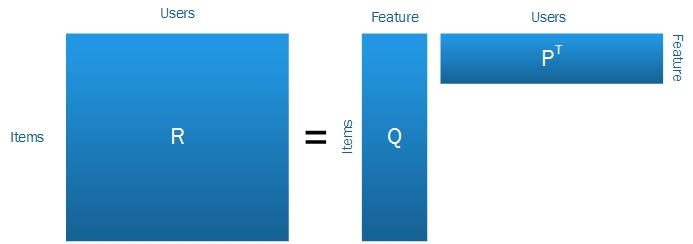
\includegraphics[width=5in]{image/matrixdecomp.jpg}
    \centering
    \caption[Matrix decomposition of the rating matrix $R$]{Matrix decomposition of the rating matrix $R$}
    \label{figure:matrixdecomp}
\end{figure}

User-item interactions are modeled as inner products in that space. For a given
item $s$, the elements of $q_{s}$ measures the extent to which the item
possesses those factors, positive or negative. Likewise, for a given user $c$,
the element $p_{c}$ measures the extent of interest that user has in items that
are high on the corresponding factors. The resulting dot product $\hat{u(c,s)}$
captures the overall interest of the user in the characteristics of the items.

\begin{equation}
u(c,s) = p_{c}^{T}q_{s} = \sum_{k=1}^{f} q_{sk}p_{kc}
\end{equation}

The problem then, is to discover the user factor matrix $P$ and the item factor
matrix $Q$ such that their product approximates the original rating matrix $R$.

\begin{equation}
R \approx Q \times P^{T} = \hat{R}
\label{equation:dotproduct}
\end{equation}

To learn the factor vectors the system minimizes the regularized square error
on the set of known rating $K$.

\begin{equation}
\label{equation:minimize}
min_{q, p} = \sum_{(c,s)\epsilon K} (u(c,s) - p^{T}_{c}q_{s})^{2} + \lambda ( \Vert q_{s} \Vert ^{2} + \Vert p_{c} \Vert ^{2})
\end{equation}

However, it is important to remember that our goal is generalize beyond the
observed ratings, in a way that we can predict future unknown ratings. The
system should therefore avoid overfitting the data by regularizing the learned
parameters, whose magnitudes are penalized. $\lambda$ controls the extent of
regularization, and much like $f$, often determined by cross-validation. Two
possible approaches to minimizing Equation \ref{equation:minimize} is to use
Stochastic Gradient Descent or Alternating Least Squares \citep{Koren2009}.\newline

Consider the following example where we have the following rating matrix R
shown in Table \ref{table:ratingMatrix} containing the rating of four users $C$
for four items $S$, giving us a $C \times S$ matrix with explicit ratings on a
  scale from 1 to 5.

\begin{figure}[H]
	\centering
	$
	\begin{bmatrix}
		5.00    & 5.00  & 2.00 & -    \\
		2.00    & -     & 3.00 & 5.00 \\
		-       & 5.00  & -    & 3.00 \\
		3.00    & -     & -    & 5.00
	\end{bmatrix}
	$
	\caption{Rating matrix $R$}
	\label{table:ratingMatrix}
\end{figure}

Given that $f = 3$, we might end up with the following matrix $P$ and $Q$

\begin{figure}[H]
\centering
$
\begin{bmatrix}
1.81    &1.62   &0.74\\
2.66    &1.71   &-1.08\\
1.73    &-0.23  &0.78\\
3.16    &-0.24  &0.90
\end{bmatrix}
$
\caption{User factor matrix $P$}
\end{figure}

\begin{figure}[H]
\centering
$
\begin{bmatrix}
1.12    &	1.49   &	0.48\\
1.31    &	-0.52  &	0.59\\
1.13    &	0.67	&	-0.52\\
1.39    &	0.05	&	0.45
\end{bmatrix}
$
\caption{Item factor matrix $Q$}
\end{figure}

Equation \ref{equation:dotproduct} then gives us the following rating prediction matrix $\hat{R}$.

\begin{figure}[H]
\centering
$
\begin{bmatrix}
4.79    &5.01   &1.97   &3.61 \\
1.97    &1.96   &2.85   &4.80 \\
2.75    &4.71   &1.40   &2.94 \\
2.93    &3.30   &2.74   &4.78
\end{bmatrix}
$
\caption{Rating prediction matrix $\hat{R}$}
\end{figure}



As you can see the values of known ratings in Table \ref{table:ratingMatrix}
are fairly similar to the corresponding ratings in the rating prediction
matrix.

\subsection{Hybrid approaches}

A term \emph{hybrid recommender systems} is used to describe any recommender
system that combines multiple recommendation techniques together to provide
recommendations. Burke et al. \cite{Burke2002} identified seven different
classes of hybrid recommender systems:

\begin{itemize}
\item Weighted: The score of different recommendation components are combined numerically.
\item Switching: Switching between recommender systems depending on the situation.
\item Mixed: Recommendations from different recommenders are presented together.
\item Feature Combination. Features derived from different knowledge sources
are combined together and given to a single recommendation algorithm
\item Feature Augmentation: One recommendation technique is used to compute a
feature or set of features, which is then part of the input to the next
technique.
\item Cascade: Recommenders are given strict priority, with the lower priority
ones breaking ties in the score of the higher ones
\item Meta-level: One recommendation technique is applied and produces some
sort of model, which is then the input by the next technique
\end{itemize}

Most commonly hybrid systems are built by combining collaborative and
content-based methods in an attempt to mitigate the limitations the approaches
suffer individually. Adomavicius and Tuzhilin \cite{Adomavicius2005} lists the
following approaches to building hybrid recommender systems:

\begin{itemize}
\item Implementing the systems separately and combining their predictions
\item Incorporating content-based characteristics into a collaborative approach
\item Incorporating collaborative characteristics into a content-based approach
\item Constructing a general unifying model that incorporates both
content-based and collaborative characteristics
\end{itemize}

\marginpar{heri-notes: Which approach relevant to this work?}

\subsection{Recommender System Challenges}

Below we briefly mention some of the main challenges one faces when working
with recommender systems.

\subsubsection{Scalability}

As the number of existing users and items blow up, traditional CF algorithms
suffer serious scalability problems. The model building phase of \emph{Traditional}
collaborative filtering methods have a complexity of O(MN) where $M$ is the number
of users and $N$ is the number of items. For systems with millions of users and items,
even a complexity of $n$ is too large. Another fundamental issue is how to embed the
core recommendation techniques in real operational systems and how to deal with massive
and dynamic sets of data produced by the interactions of users with items. Recommender
systems are expected in many cases to provide rapid recommendations online, it is
therefore also important to consider how fast the system provides recommendations.

Better scalability and improved accuracy make the item-item collaborative filtering
approaches more favourable in many cases. The computational complexity of item-to-item
based algorithms are up to two orders of magnitude faster than traditional user-based
algorithms \cite{Deshpande2004}. Dimensionality reduction techniques such as
SVD can deal with the scalability by providing more compact representations and
quickly produce good recommendations. However, most dimensionality reduction
techniques must undergo expensive matrix factorization steps.

\subsubsection{Sparsity}

In practice, many recommender systems deal with very large item collections.
This means that the number of ratings obtained is usually very small compared to the
number of ratings that it needs to predict. Efficient prediction of ratings from a small
number of examples is therefore important. The \emph{reduced coverage} problem
occurs when the number of users' rating may be very small compared to the number of items.
This may lead to that the recommender is unable to provide recommendations for a large
portion of the items. \emph{Neighbour transitivity} refers to the problem in which users
with similar tastes may not be identified due to a lack of co-rated items, making
collaborative filtering futile, since it relies on comparing users to predict unknown ratings.

\subsubsection{Cold-start}

Conceptually, the cold-start problem can be viewed as a special instance of the
sparsity problem, where most elements in a certain row or column are zero. The
cold-start problem further emphasizes the importance of the sparsity problem.
Whenever a new user or item enters the system, it is difficult to find similar
ones as there is little or no information available. New items can therefore
not be recommended until they have been recommended by a substantial amount of
users. Similarly, giving \emph{good} personalized recommendations to new users
based on a few ratings is difficult, since it does not give a good overall
picture of a users tastes and preferences. These problems are known as the
\emph{cold-start user} and \emph{cold-start item} problems.

\subsubsection{Shilling attacks}

In recommender systems where everyone can give ratings, people may give lots of
positive ratings to their own items and negative ratings to their competitors.
It is often necessary for collaborative filtering systems to introduce
precautions to discourage such kind of manipulation.

\subsection{Terminology}

\marginpar{TODO: Fjerne?}

%TODO - Any more RS related terminology that needs explaining?

\subsubsection{Explanations / Transparency}

\marginpar{heri-notes: Hvorfor har dere med dette?}

Tintarev et al. \cite{Tintarev2007} lists seven roles a that can be played by explanations in recommender systems:

\begin{itemize}
\item Transparency: Explaining how the system works
\item Scrutability: Allowing the users to tell the system it is wrong
\item Trust: Increasing user confidence in the system
\item Effectiveness: Help users make good decisions
\item Persuasiveness: Convince users to try or buy
\item Efficiency: Helping users to make decisions faster
\item Satisfaction: Increasing the ease of use or enjoyment
\end{itemize}

In collaborative filtering systems the explanations is of the form "Other users
similar to you liked this item", while in content-based style explanations, the
item's attributes which most affected the item to be recommended to the user
are illustrated. For example, in a fashion recommender, an explanation may be
of the form "This shirt was recommended because it's a Ralph Lauren who you
seem to like".
